% Chapter 2

\chapter{Introduction} % Main chapter title
\label{chapter:introduction} % For referencing the chapter elsewhere, use \ref{Chapter1} 

\section{Background and Problem Statement}
The biomechanical characterization of soft tissues has gained attention
in medical research \cite{Cox2006}, in areas such as medical image analysis and visualization.
For many years, the obtained medical diagnoses were often based on the assumptions of experts or 
their accumulated experience. While this information have proven to be useful in general, 
these methods have limitations in cases where quantifiable data is necessary, specifically for computer-assisted systems, e.g,
medical diagnosis, therapy, and training \cite{Kauer2002}.
To gather the material data, e.g., elasticity, stiffness, response under deformation and temperature, it is required 
to gain access to the soft tissues and perform \textit{in vivo} testing experiments. 
However, obtaining accurate biomechanical data can be challenging 
due to the invasive nature of the procedures and the difficulty in maintaining constant and reproducible internal or external factors  
in experimental configurations \cite{Carter2001}.\\

%Precise knowledge about the biomechanical characterization of soft tissues has received attention
%in medical research, e.g., medical image analysis and visualization.
%For many years, the obtained medical diagnosis have come from assumptions of experts or 
%accumulated experience. This information, although proven to be useful, has its limitations 
%when computed-assisted systems like, medical diagnosis, therapy, and training, rely on 
%more quantifiable data \cite{Kauer2002}. To gather this data, it is important to gain access
%to the tissues and perform in vivo testing experiments. For organs, this procedure is nearly 
%impossible to achieve, due to the involvement of an invasive procedure, and the lack of constant
%and reproducible external and internal factors. \\ 
Especially, when it comes to internal organs, obtaining reliable data for examination after their 
extraction is difficult because the material properties can vary between samples or testing 
locations on the same organ \cite{Chai2013}. This is due to the influence of various factors such as changes in blood pressure, changes in material properties 
over time, symptoms of disease, and more. In addition, another problem is the lack 
of replication, due to the use of different individuals' organs, which introduces more external
factors into the equation. Moreover, given a tissue sample, it is difficult to properly 
characterize the material due to its anisotropic property, which can lead potentially
 to inaccuracies in the result \cite{Cox2006}.

%Particularly in the case of internal organs, one of the challenges associated with their extraction 
%is that some material properties may change despite examination of the same sample. Their biomechanical properties 
%depend on other factors, such as changes in blood pressure, changes in material properties 
%over time, symptoms of disease, and more. In addition, another problem is the lack 
%of replication, due to the use of different individuals' organs, which introduces more external
% factors into the equation. Moreover, given a tissue sample, it is difficult to properly 
% characterize the material due to its anisotropic property, which can lead to inaccuracies in the result.\\

In the situation where the material data can be collected in a constant, fast and reliable
process, a material model can be established and the computer-aided systems can predict 
the mechanical behavior of soft tissues, providing preoperative calculations. 
This demonstrates the importance of material data collection and material model development, 
especially in the context of computational models such as engineering simulation models created finite 
element analysis (FEA) software and their medical applications in medical devices, surgical 
procedures, and training softwares \cite{Carter2001}. By using accurate material models, the accuracy of the simulation 
can be improved, aiding in a better understanding and predicting a soft tissue response 
to external stimuli \cite{Zhang2014}, making them more useful in medical research and other related applications.\\

\section{Objective and Scope of the Study} 

Soft materials, characterized by low elastic moduli and high sensitivity to external stimuli,
frequently experience large deformation and display nonlinear responses \cite{Zhang2014}, making 
the finite element method (FEM) a common approach for analyzing these materials and solving continuum mechanical problems. 
Although FEM facilitates the analysis of complex structures with complex material 
behavior, simulating such materials requires high computational costs.\\

The main objective of this study is to identify the key parameters of soft materials and their 
influence on the development of a material model based on inverse finite element method (iFEM) approach. 
By identifying these key parameters, an attempt is made to approximate the behavior of 
complex materials through a simplified material model and
assess its potential future applications in medical research and its use with organs.\\

To achieve this goal, an experimental configuration will be selected, and a computational model will be 
developed to use an iFEM approach to identify the key material parameters of the given soft material. 
With this method, it was possible to match the results of the computational model to the experimental 
data, and validate the model with additional data points. 

The objective of this study is to develop a framework that identifies the essential material parameters of soft materials 
and evaluates their limitations and impact on a validated model, which can describe nonlinear material behavior.
By contributing to this framework, the study aims to accelerate the development of material models for practical 
applications in medical research and development.
%---------------------------------------------------------------------------------
\section{State of the Art}

This section reviews the state of the art relevant to this study. First, the experimental characterization 
techniques are reviewed, including methods for obtaining mechanical and viscoelastic properties.
This is followed by the description of different approaches to describe the material model for different soft 
materials. Then, the iFEM, which is one method to identify material parameters from experimental data, 
will be explained. Finally, the standard verification and validation process used in computational 
solid mechanics for medical devices based on the American Society of Mechanical Engineering (ASME) guidelines 
will be discussed. The goal of this chapter is to provide a comprehensive overview of the current methods use in 
the field and the identification of limitations and gaps in the current state of knowledge. %maybe take out?

%--------------------------------------------------------------------------------------------------
\subsection{Experimental Characterization for Soft Materials}
\label{subsection:experimentalcharacterization}
%In this section, you can discuss the various experimental techniques that have been used to characterize 
%the mechanical properties of soft materials. You can talk about traditional mechanical testing methods such 
%as tensile and compressive testing, as well as more specialized techniques such as indentation testing, 
%shear testing, and dynamic mechanical analysis. You can also discuss the advantages and limitations of 
%each technique, and highlight any recent advancements in experimental characterization.
%material testing
Experimental testing is a key approach to obtaining information about the mechanical behavior of soft materials.
In order to characterize the mechanical behavior of a test specimen, the most common method
method is to mechanically load the specimen and measure the response of the force against 
the displacement \cite{Bergström2015}. Soft materials are commonly applied 
for tissue engineering applications, however, challenges arise for the 
design of experimental design due to their elastic modulus range ($\SI{}{\kilo \pascal}$) and complex
mechanical properties \cite{Liu2009}.\\

%Soft materials challenges in experimental deign
%-Soft synthetics materials like soft gels are often used for tissue engineering applications.
%However, due to their 

%- Soft synthetics materials like soft gels are one example for soft synthetic materials. These
%are commomly applied for tissue engineering applications. Nevertheless, due to their elastic 
%modulus range (kPa) present some challenges for the design of experimental testing \cite{Liu2009}.

\subsubsection*{Uniaxial Tension Testing}

Uniaxial tension testing are widely employed to determine an stress-strain relationship.
For uniaxial tension cases, a specimen is typically loaded by gripping the ends while applying 
tension, and the deformation is usually measured with a strain gauge \cite{Bergström2015}.
This kind of testing focuses on the central region of the specimen to evade complication arising from 
"edge effects". An homogeneous deformation in the central region is usually expected for this kind of testing, 
which simplifies the boundary problem and ensures that the measurements represents valid stress-strain values.
However, there are two key limitations for uniaxial testing when testing soft materials; first, 
it may not be suitable when complex boundary conditions arise and is not possible to contro the 
experimental condition entirely \cite{Seshaiyer2003}. Second, these tests are inadequate to 
fully characterize the anisotropic behavior of these materials \cite{Cox2006}.\\

In a study made by \citet{Kanyanta2010}, the authors investigated the behavior of an ether-based polyurethane 
elastomer for the creation of mock arteries. Polyurethane was ideal for this application due to 
its high elasticity and resilience and adaptability to various shapes and sizes. Uniaxial tensile tests on 
dumbbell-shaped specimens were conducted, divided into three groups based on the strain rate.

\begin{figure}
        \centering
    
        \begin{subfigure}[b]{0.45\textwidth}
        \centering
        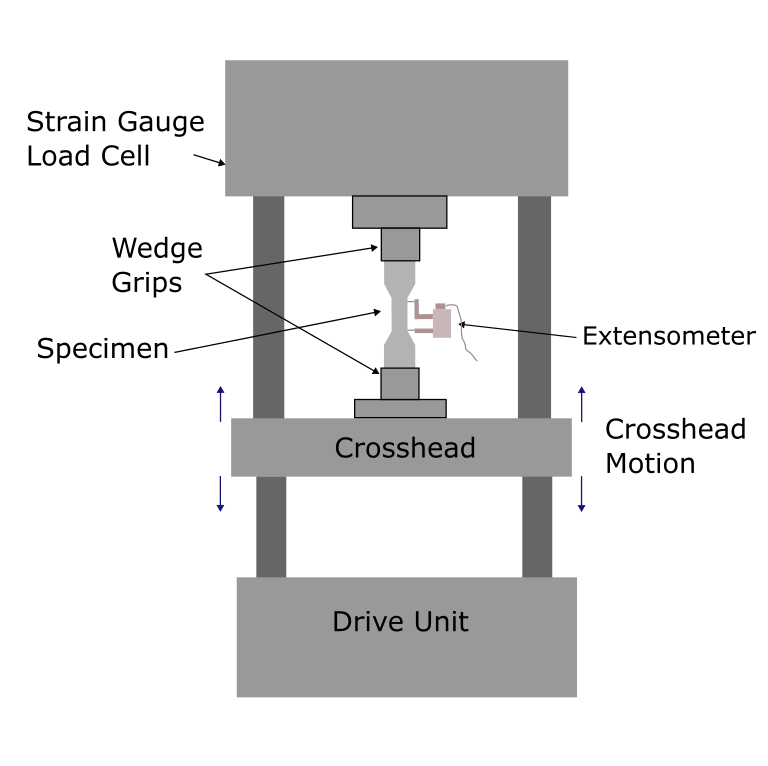
\includegraphics[width=\textwidth]{Images/chapter1/uniaxialtension.png}
        \caption{Low strain rate test with a standard tensile machine}
        \label{fig:subfiglow}
        \end{subfigure}
        \hfill
        \begin{subfigure}[b]{0.45\textwidth}
        \centering
        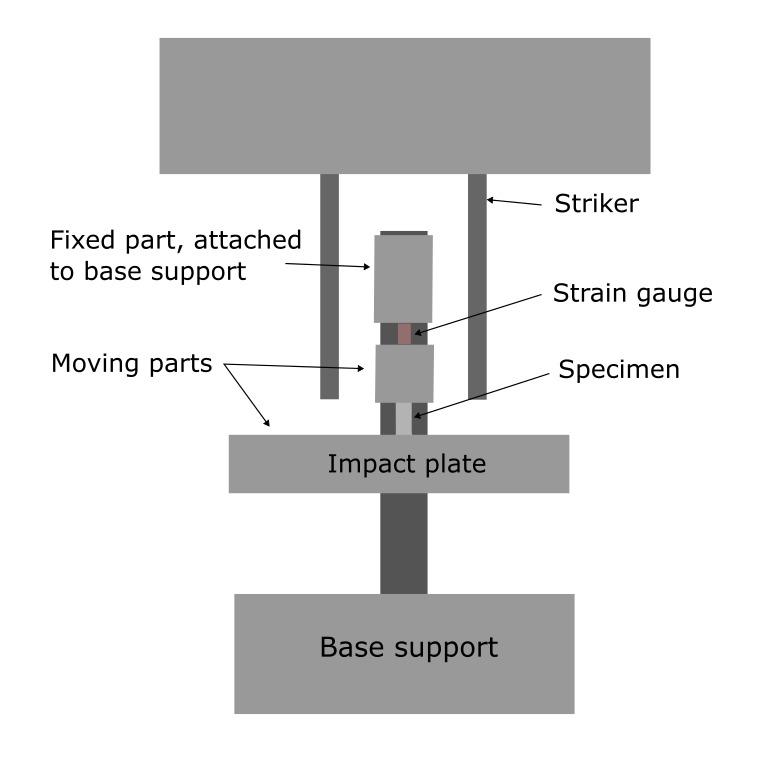
\includegraphics[width=\textwidth]{Images/chapter1/uniaxialintermediate.png}
        \caption{Intermediate strain rate test with a falling weight impact tester}
        \label{fig:subfiginter}
        \end{subfigure}
        \vspace{0.5cm}
        \begin{subfigure}[b]{0.7\textwidth}
        \centering
        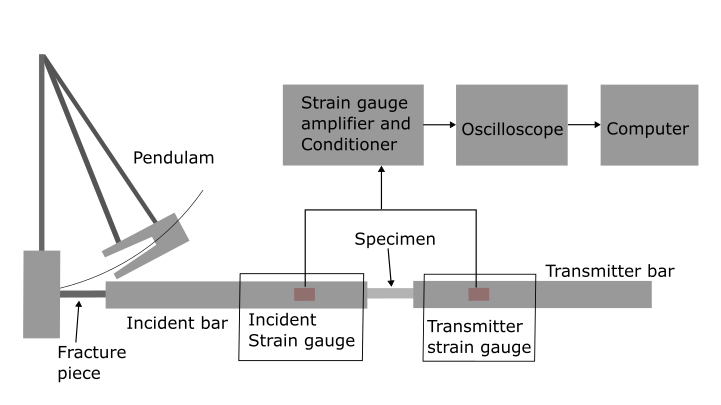
\includegraphics[width=\textwidth]{Images/chapter1/uniaxialhigh.png}
        \caption{High strain rate test with a split Hopkinson pressure bar in tension}
        \label{fig:subfighigh}
        \end{subfigure}  
        \hspace{0.3cm}

        \caption[Uniaxial tensile testing of ether-based polyurethane, \citet{Kanyanta2010}]{Uniaxial tensile testing: Diagram of three tensile testing of an ether-based polyurethane elastomer specimen done with three different experiment configurations for different strain rate analysis. Diagrams are based on the experiments of made by \citet{Kanyanta2010}.}
        \label{fig:uniaxialkan}
\end{figure}

For the low strain rate tensile tests ($< \SI[per-mode = symbol]{1}{\per \second}$), a standard Instron machine was utilized, as illustrated in Figure 
\ref{fig:subfiglow}. Intermediate strain rate tensile tests (between $\SI[per-mode = symbol]{1}{\per \second}$ and $\SI[per-mode = symbol]{100}{\per \second}$) 
were performed using a drop-weight tester (Fig. \ref{fig:subfiginter}). Load measurements were recorded with a calibrated strain gauge, 
with the zero position established at the striker and impact plate's initial contact point.
High strain rate tests ($>\SI[per-mode = symbol]{100}{\per \second}$) were conducted with a split Hopkinson pressure bar in tension, as shown in Figure \ref{fig:subfighigh}.
A swinging pendulum generated a tensile pulse, propagating along the bar into the specimen. Utilizing 
the transmitted and reflected strain signals and using the classical Kolsky analysis the specimen stress
\begin{align}
        \sigma(t) = E\frac{A_b}{A_s}\epsilon_t(t) \, ,
\end{align}
and the strain
\begin{align}
        \epsilon(t) = \frac{-2C_b}{l_s} \int_{0}^{t} \epsilon_r(t) dt \, ,
\end{align}

were calculated. Here, $A_b$ is bar's cross-sectional area, $A_s$ the specimen's cross-sectional area,
$\epsilon_t$ refers to the transmitted strain signal, $\epsilon_r$ is the reflected strain signal,
$l_s$ is the specimen gauge length, and $C_b$ is the wave speed through the bar.
Low strain rate tests were conducted under dry-room temperature, wet-room temperature, and wet at $\SI{37}{\degreeCelsius}$. 
Intermediate and high strain rate tests were performed exclusively under dry-room temperature conditions.\\

Test results demonstrated that ether-based polyurethane elastomer specimens were highly sensitive to 
temperature and humidity, as the material softened with increased levels of these factors. Young's 
modulus values for dry-room temperature setup $\SI{7.4}{\mega \pascal}$, decreasing to $\SI{5.3}{\mega \pascal}$ 
and $\SI{4.7}{\mega \pascal}$ for the wet-room temperature and wet conditions, respectively.
Moreover, the polyurethane exhibit varying Young's modulus values under dry-room temperature, depending 
on the elastomer's composition, with values ranging from $\SI{3.6}{\mega \pascal}$ to $\SI{14.8}{\mega \pascal}$.

The material displayed minimal strain rate dependency at low strain rates, but exhibited moderate 
strain rate sensitivity at intermediate and high strain rates, where the Young's modulus ranged between 
$\SI{8}{\mega \pascal}$ and $\SI{12}{\mega \pascal}$. However, for strains below $\SI{20}{\percent}$, the 
outcomes showed repeatability across all strain rates tests. 

For strain rates found in arteries around $<\SI[per-mode = symbol]{2}{\per \second}$, the variation of the
Young's modulus was insignificant and this could be assumed to be constant. This study demonstrated 
that it is important to measure the properties of the elastomer under similar condition to the
intended application, as properties varies under different conditions.

\subsubsection*{Uniaxial Compression Testing}
Compression tests are also widely utilized to determine the stress-strain response and 
usually involve placing the specimen in between two plates and compressing the material (Fig. \ref{fig:compressiondiag}).
The stress-strain response derived from this kind of testing serves in determining the deformation 
characteristics of the material including the fatigue and fracture resistance. 
Uniaxial compression tests may be affected by the interface friction between the specimen and 
the loading plates, leading to a nonhomogeneous deformation state, e.g., barrelling \cite{Bergström2015}.\\

\begin{figure}%
        \centering
       \quad
       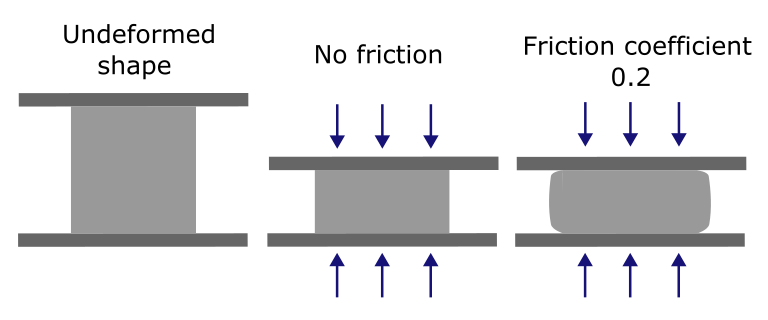
\includegraphics[width=10cm]{Images/chapter1/compressiondiag.png}%
       \caption[Uniaxial compression testing setup based on the book by \citet{Bergström2015}]{Uniaxial compression testing: Diagram of typical compression setup and influence of interface friction on the deformed specimen shape. Illustration is based on the "Mechanics of Solid Polymers" by \citet{Bergström2015}.}%
       \label{fig:compressiondiag}%
\end{figure}

\citet{Drass2018} conducted a uniaxial compression test, showing that the lubrication was 
crucial for an homogenous stress and strain distribution. The specimen tested was made from Transparent Structural 
Silicone Adhesive (TSSA), a rubber-like material commonly used in laminated connections within glass structures.
In this study homogeneous and inhomogeneous experiments were performed, as the goal was to determine an 
experimental setup, which ensured an homogeneous stress and strain distributions for the identification of material parameters \cite{Drass2018}.

The specimen was compressed with perfect slippage, where the plates and the specimen were lubricated 
before testing to ensure a frictionless support. A constant speed of $v_{UC}=\SI[per-mode = symbol]{0.174}{\milli \m\per \minute}$
was used for this test with a saBesto HHS 5000 machine. The compression test were consucted until a strain $\epsilon=\SI{0.6}{}$ 
was reached, as the standard deviation for large compression strain ($\epsilon > \SI{0.5}{}$) was too large.
The test presented challenges in maintaining the lubrication throughout the test, as it tended to be 
pressed out between the test specimen and the pressure plates, resulting in a increased friction. 

The results of this experiment were processed to identify hyperelastic material parameters using standard 
fitting routines and inverse methods. The test suggested that only stress-strain response up to a strain value of 
$\epsilon=\SI{0.5}{}$ should be considered for the indentification of the TSSA material parameters, as 
the friction's impact can be neglected for smaller strains.\\

In comparison, for a biomaterials, e.g., human soft tissues, a compressive testing of cartilage was conducted by \citet{Griffin2016}. 
This study aimed to provide a protocol were compressive and tensile properties of human soft tissues can be evaluated 
and characterized with minimal destruction. By understanding these material's properties and calculating the Young's 
elastic modulus, it would be possible to obtain a benchmark for creating suitable tissue-engineered substitutes \cite{Griffin2016}. 

The mechanical response of cartilage is highly dependant to the fluid's flow through the tissue. The methods for compression 
testing can vary with confined or unconfined specimen, and the most prevalent, indentantion (Fig. \ref{fig:compressiontypes}).
In the unconfined compression the cartilage is pressured using a non-porous plate onto a non-porous chamber, 
leading to a predominatly radial fluid flow. For the confined compression the sample was placed in a sealed, 
fluid-filled impermeable chamber and loaded with a porous plate, making the fluid flow restricted to a vertical direction.
Finally, the indentation testing employed a smaller indenter applied to the sample's surface perpendicularly, ensuring 
uniaxial compression and minimizing shear loading. All test were conducted in a 
hydrated environment and the cartilage was submerged in phosphate-buffered saline before and during the test to maintain 
the hydration. With the latest compression testing type it was possible to identify elastic and viscoleastic properties 
of the sample \cite{Griffin2016}.

\begin{figure}%
        \centering
       \quad
       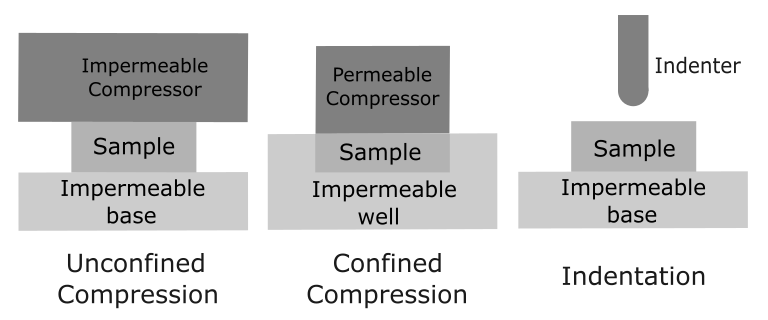
\includegraphics[width=10cm]{Images/chapter1/compressiontypes.png}%
       \caption[Uniaxial compression testing methodologies by \citet{Griffin2016}]{Uniaxial compression testing: Illustration of different compression methodologies for a cartilage specimen. Unconfined compression, confined compression and Indentation. Diagrams are based on the methodologies showed by \citet{Griffin2016}.}%
       \label{fig:compressiontypes}%
\end{figure}

%------------------------------------------------------------------------
\subsubsection*{Indentation}
Indentation testing, including micro and nanoindentation, is a popular method for characterizing 
the mechanical properties of soft materials \cite{Wu2016}. One of the main advantages of 
indentation testing is that it requires minimal sample preparation and it is often a 
nondestructive technique, which allows the preservation of the geometry and tissue's architecture \cite{Shi2019}.
Furthermore, indentation is useful where more traditional testing techniques such as 
uniaxial or biaxial testing, are not possible to employ, 
and can also be utilized to evaluate nonlinear properties, e.g., viscoplastic responses\cite{Bergström2015}.\\

Despite these advantages, there are challenges when using indentation to 
characterize soft materials. First, a stress-strain response is difficult to
obtain due to the complex boundary conditions, which introduces an inverse problem 
for the identification of material parameters \cite{Shi2019}. Second, many of the current 
indentation configurations assume material isotropy, which may not be the case for biomaterials \cite{Feng2017}.
In addition, determining the mechanical properties of soft materials locally or at small scales is still difficult to achieve \cite{Zhang2014}.


The usual indentation testing setup is shown in Figure \ref{fig:Nanoindentation}, in this case a 
system applies a certain force to an attached indenter rod where and specific 
indenter tip. After the indenter tip goes to a determined displacement, 
it is possible to obtain a load-displacement curve.
The deformation can be measured through an capacitance gauge or also optically, via laser measurements \cite{Bergström2015}.\\

\begin{figure}[th]
        \centering
        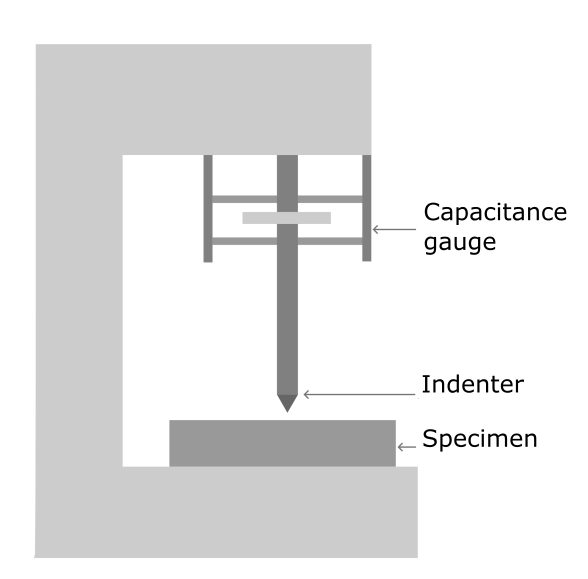
\includegraphics[width=7cm]{Images/nanoindentationbigletter}
        \caption[Nanoindentation experiment diagram by \citet{Bergström2015}]{Nanoindentation experiment setup diagram with an indenter tip attached to a rod and a polymer as specimen. Diagram is based on the "Mechanics of Solid Polymers" by Bergström \cite{Bergström2015}.}
        \label{fig:Nanoindentation}
\end{figure}

In a study made by \citet{Zhang2014} an investigation of spherical indentation on hyperelastic 
soft materials was conducted. The material utilized in the experiments was polydimethylsiloxane (PDMS),
with was prepared and cured in a cylindrical mold and cured at $\SI{60}{\degreeCelsius}$ for eight hours. 
The ElectroForce 3100 was used to measuring the mechanical properties of PDMS for tensile and 
indentation tests. Tensile tests were performed to identify the initial shear modulus and 
locking stretch and their results compared with the indentation tests \cite{Zhang2014}. 
For the indentation tests an spherical indenter with a $\SI{3}{\milli \m}$ radius with a similar configuration 
shown in Figure \ref{fig:Nanoindentation} was used. The measurements were done under room temperature and 
a humidity of $\SI{50}{\percent}$ with a loading rate of $\SI[per-mode = symbol]{2}{\milli \m\per \second}$ and 
a indentation depth of $\SI{3}{\milli \m}$. Six measurements were carried out at different 
locations on the specimen, generating an indentation load-displacement curves. 
Moreover, the initial shear modulus was determined using fitted results of the load-depth curves to 
the Hertzian and hyperelastic solution developed in the study.

The results exhibited that the determination of the initial shear modulus was possible but a 
certain depth depence coudl be observed. However, a locking stretch could not be analyze due to the 
sensitivity of these parameters to experimental data noise \cite{Zhang2014}.\\

For an application with biological tissues \citet{Carter2001} performed indentation experiments on 
human and porcine organs for its application in realistic computer-based simulators 
for minimal access surgery (MAS) training. 
This study investigated the stress-strain data pig spleen and liver for \textit{ex vivo} experiments, 
along with human liver for \textit{in vivo} experiments from volunteers patients undergoing a minor 
surgery. For the \textit{ex vivo} experiment a static indentation setup was used as shown in Figure 
\ref{fig:carter1}, where the specimens were placed on a flat surface. A force was applied 
manually with a winding mechanism at constant rate of $\SI[per-mode = symbol]{1}{\milli \m\per \second}$ 
with a rounded indenter with a diameter of $\SI{4.5}{\milli \m}$. Ten measurements were 
carried out on each tissue sample and the load-displacement measurements were 
gathered with a computerized system with a sampling rate of $\SI{15}{\hertz}$.\\

\begin{figure}
        \centering
        \begin{subfigure}[b]{0.45\textwidth}
        \centering
        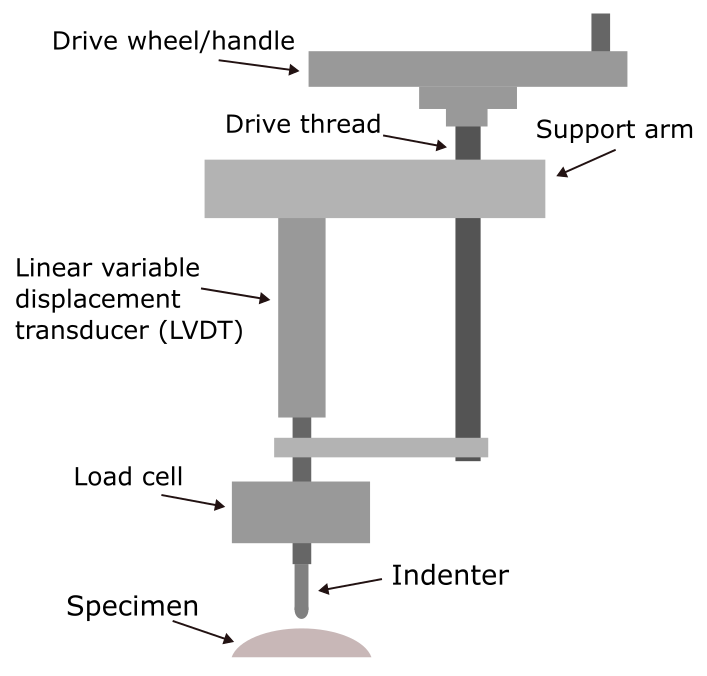
\includegraphics[width=\textwidth]{Images/chapter1/indentation1carter.png}
        \caption{Static indentation configuration used for \textit{ex vivo} indentations tests. Indenter advances against the tissue by rotating the wheel}
        \label{fig:carter1}
        \end{subfigure}
        \hfill
        \begin{subfigure}[b]{0.45\textwidth}
        \centering
        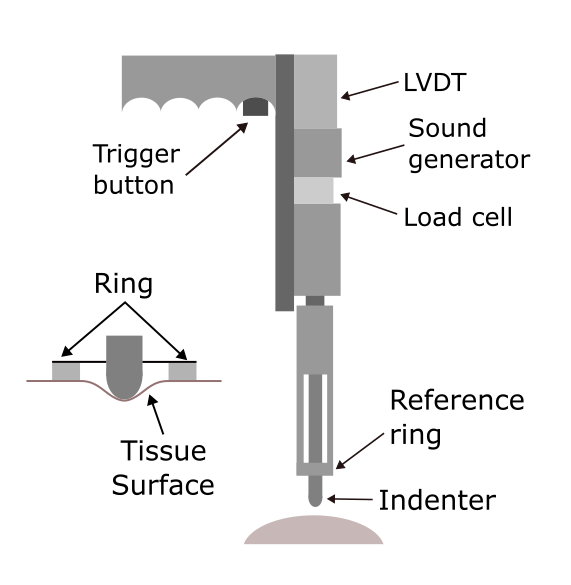
\includegraphics[width=\textwidth]{Images/chapter1/indentation2carter.png}
        \caption{Mobile indentation configuration with outer ring case attached for stabilization of the indentation test.}
        \label{fig:carter2}
        \end{subfigure}
        \hspace{0.3cm}
        \caption[Indentation setup of synthetic and biological tissues by \citet{Carter2001}]{Indentation testing: Diagram of static and mobile indentation tests, indenters were attached to a load cell, which was connected to a displacement transducer. Diagrams are based on the study of made by \citet{Carter2001}.}
        \label{fig:indentationcarter}
\end{figure}

The \textit{in vivo} experiments were carried out using a hand-held compliance probe. To achieve 
an overall consistency of the measurements the same surgeon performed the experiments. 
In addition to maintain consistent indentation depth of $\SI{5}{\milli \m}$ the indenter was 
surrounded with a reference ring to provide stability in the measurements (Fig. \ref{fig:carter2}). The force 
exerted by the weight of the ring was around $\SI{0.5}{\newton}$, while the friction force 
between the ring and the surface tissue was below $\SI{0.05}{\newton}$, making it a negligible 
effect. The probe was positioned on the tissue and when the desired indentation depth was 
indicated with an audible signal. The indentation rate for this configuration ranged 
from $\SI[per-mode = symbol]{3}{\milli \m\per \second}$ to $\SI[per-mode = symbol]{4}{\milli \m\per \second}$ and 
six measurements were carried out on each patient.

The results were analyzed using MATLAB and showed highly nonlinear stress-strain behavior and large variances. 
For the reduction of these variances due to the inhomogeneity of the materials and changes over time, 
the average of the repeated measured was calculated. The measured elastic moduli of pig 
spleen and liver was $\SI{0.11}{\mega \pascal}$ and $\SI{4}{\mega \pascal}$ respectively, and 
for the human liver about $\SI{0.27}{\mega \pascal}$ was measured. However, a 
diseased liver showed a higher elastic modulus of $\SI{0.74}{\mega \pascal}$ \cite{Carter2001}.
%-------------------------------------------------------------------------------------------------
\subsubsection*{Aspiration Experiment}

Tissue aspiration experiments was a method introduced by \citet{Kauer2002} for determining 
the material parameters of biological soft tissues \textit{in vivo}.
In this study the method was validated with a synthetic material, Silgel, a very 
soft gel-like material with similar properties to biological soft tissues. 
This material was ideal to use it for the validation of the 
aspiration method before applying it to human tissues \cite{Kauer2002}.

The biological sof tissue used in this paper was human uterus. This tissue was selected 
because it possesses a complex, multilayered structure with anisotropic properties. 
Moreover, hysterectomy (removal of the uterus) is common surgical procedure, which 
provides a good chance to perform measurements before and after the removal of the organ.\\

This method introduced an aspiration tube which is put against the 
soft tissue, generating a vacuum a causing the deformation of the tissue (Fig. \ref{fig:aspiration} ). 
An advantageous feature of this experimental technique is that 
it can be perfomed \textit{in vivo} and \textit{ex vivo}.
With the help of a mirror placed next to aspiration hole, the reflection 
of the side-view of the tissue can be captured with a video camera.
This camera captures the images of the iluminated surface of the material and the 
aspiration pressure is captured through a sensor. Through this process the captured 
profile of the tissue is obtained and this can be used to characterize the deformation 
and analyze the viscoelastic properties of the soft tissue \cite{Kauer2002}.

\begin{figure}[th]
        \centering
        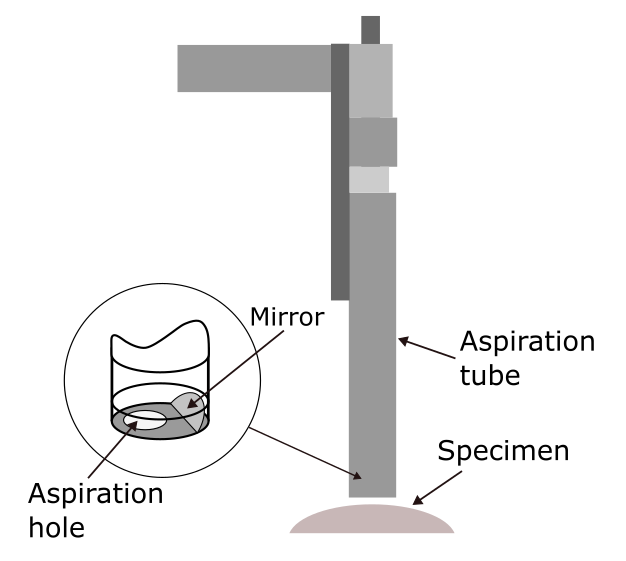
\includegraphics[width=7cm]{Images/chapter1/aspirationkauer.png}
        \caption[Aspiration experiment by \citet{Kauer2002}]{Aspiration experiment setup: Diagram showing aspiration tissue vertically positioned to the target tissue, inside of the tube a mirror reflects the side view of the tissue to the video camera on top. Diagram based on the research of \citet{Kauer2002}.}
        \label{fig:aspiration}
\end{figure}

The main benefits in comparison to more traditional experimental techniques are, 
the well-defined mechanical boundary conditions during the experiment are executed, 
large deformation experiments can be assessed, and the viscoelastic
properties of the tissue can be analyzed for real surgical procedures due to 
the time dependent resolution of the deformation.

The results from these experiments corroborates that the development of experimental designs for
biological soft tissues and its application in real-world scenarios is essential to understand 
their mechanical behavior and make advance in medical research.

%---------------------------------------------------------------------------------
\subsection{Material Modeling of Soft Materials}
\label{subsection:materialmodeling} 

Material models, such as linear elasticity and hyperelasticity play a crucial role for the characterization 
of material properties, as these describe a relationship that represents how a material behaves, e.g, 
the stress response for an applied strain, or the heat transfer for a defined temperature gradient.
For the case of soft materials, hyperelastic models are usually 
useful candidates, as these models can often predict the behavior of complex materials under certain limitations.
Moreover, hyperelastic models can be used as a foundation for more advance models like 
viscoelastic and viscoplastic models \cite{Bergström2015}. 

Hyperelastic models are useful due to their ease of use and calibration, accessibility in major commercial FE softwares, 
and computational efficiency. However, these models possess some limitations, such as being 
accurate for monotonic loading, and not capturing rate effects, i.e., viscoelasticity, or 
hysteresis during cyclic loading \cite{Bergström2015}.

In this subsection, linear elasticity and hyperelasticity constitutive models will be presented 
based on the overview made by \citet{Bergström2015}, followed by examples from the research 
papers from the Subsection \ref{subsection:experimentalcharacterization} to confirm the relevance of these 
models for medical research.

\subsubsection*{Linear Elasticity}
This model is the most basic approach to represent the small strain of the mechanical behavior 
of solid polymers, with isotropic elasticity being its most elementary form \cite{Bergström2015}.
In isotropic elasticity, stress is proportional to the applied strain and independent of the material's 
orientation. Hooke's law is frequently the constitutive equation for an elastic material, and one form 
\begin{align}
        \epsilon_{ij} &= \frac{1 + \nu}{E} \sigma_{ij} - \frac{\nu}{E} \sigma_{kk} \delta_{ij} \, ,
        \label{eq:linearelasberg}
\end{align}  
was presented by \citet{Bergström2015} to define a strain-stress relationship, where the indices $i$ and $j$ take the values of 
$\SI{1}{}$, $\SI{2}{}$, and $\SI{3}{}$, $\epsilon_{ij}$ and $\sigma_{ij}$ are the strain and stress tensors, and
\begin{align}
        \delta_{ij} = \begin{cases} 
                        1, & \text{if } i=j, \\
                        0, & \text{otherwise},
                      \end{cases}
\label{eq:kronecker}
\end{align}
represents the Kronecker delta function. Similarly, the stress 
\begin{align}
        \sigma_{ij} = 2\mu\epsilon_{ij} + \lambda\epsilon_{kk}\delta_{ij} \, ,
        \label{eq:sigmalinearberg}
\end{align}
can be determined in terms of the strain using Hooke's Law. Key parameters in Equations \ref{eq:linearelasberg}
and \ref{eq:sigmalinearberg} include the Young's Modulus $E$, Poisson's ratio $\nu$, the shear modulus $\mu$, 
and the Lame's constant $\lambda$. 
The linear elastic constitutive theory can be formulated with the identification of two material parameters,
which can be determined through experimental data. After identifying these two parameters, it is possible to  
calculate any other constants. A typical experimental method to identify and calibrate a pair of parameters is the uniaxial tension 
test, where the stress-strain response identifies $E$ and $\nu$.
A significant drawback of using a linear elastic model to predict the mechanical behavior of soft polymers is 
that these materials exhibit linear behavior only within small strains and a limited range of strain-rates and 
temperatures \cite{Bergström2015}. 

\subsubsection*{Anisotropic Elasticity}
Anisotropic elasticity is an extension of linear elasticity theory that considers the anisotropic 
behavior of the material, as is usually the case for biopolymers. The strain $\epsilon_{ij}$ and stress $\sigma_{ij}$ 
\begin{align}
        \epsilon_{ij} &= S_{ijkl} \sigma_{kl}, \label{eq:strainanisotropic}\\
        \sigma_{ij} &= C_{ijkl} \epsilon_{kl}, \label{eq:stressanisotropic}
\end{align}
can be written using Hooke's Law for an anisotropic material. These equations 
show that the stress and strain tensor are linearly dependent on each other by a linear stiffness $C_{ijkl}$ 
or compliance tensor $S_{ijkl}$. The stiffness and compliance tensors possess $\SI{81}{}$ components and 
since the stress and strain tensors are symmetrical, the independent components of $S$ and $C$ can be then reduced 
to $\SI{36}{}$ components. Depending on the degree of anisotropy, these matrices can be further simplified. 

\subsubsection*{Hyperelasticity}
Hyperelastic models are an extension of linear elasticity that accounts for nonlinearity 
and large strain predictions. These models have been widely developed over the years and 
are available in various FE softwares. Hyperelastic models are very important in modeling 
soft tissues, as they can be sometimes connected to the micromechanisms driving the 
deformation behavior of the material \cite{Bergström2015}. Common hyperelastic models include the 
Neo-Hookean, Mooney-Rivlin and Ogden models.\\

\textbf{Neo-Hookean Model}\\

The Neo-Hookean (NH) model consists of a simple hyperelastic model based on the shear 
modulus $\mu$ and the bulk modulus $\kappa$. This model can be used for compressible 
and incompressible deformations, with the compressible version often being more 
practical for finite element simulations. The NH model is primarily used for 
solid, rubber-like materials characterized by an almost incompressible behavior. 
Because of this characteristic, the actual value has a minimal effect on the response 
of the observed material \cite{Bergström2015}.

The NH model is like other hyperelastic models, specified by its Helmholtz free energy per unit 
reference volume
\begin{align}
        \psi(I_1^*,J) = \frac{\mu}{2}(I_1^* - 3) + \frac{\kappa}{2}(J - 1)^2 \, ,
        \label{eq:helmholtzNH}
\end{align}
where $I_1^*$ is the distortional first invariant, and $J$ the Jacobian of the deformation gradient \cite{Youssef2022}.
This equation is inadequate for the accurate description of large-strain nonlinear responses. 
In addition, this equation is not dependent on the second invariant $I_2^*$, which limits the 
stress prediction for biaxial loading.

The Cauchy stress for compressible NH model can be expressed as \cite{Youssef2022}
\begin{align}
        \sigma = \frac{\mu}{J}\text{dev}[\boldsymbol{b}^*] + \kappa(J-1)\boldsymbol{I} \, ,
        \label{eq:cauchystressNHcomp}
\end{align}
where $\boldsymbol{b}^*$ left Cauchy-Green strain tensor, and $\boldsymbol{I}$ is the identity matrix. 
The Cauchy stress expressions for uniaxial, planar and biaxial deformations for incompressible NH models are
\begin{align}
        \sigma_{\text{uniax}} &= \mu(\lambda^2 - 1/\lambda), \label{eq:uniaxNH} \\
        \sigma_{\text{planar}} &= \mu(\lambda^2 - 1/\lambda^2), \label{eq:planarNH} \\
        \sigma_{\text{biaxial}} &= \mu(\lambda^2 - 1/\lambda^4), \label{eq:biaxialNH}
\end{align}
respectively. In these equations, $\lambda$ represents the stretches of the deformation \cite{Youssef2022}.
An alternative formulation of the NH model, where the stress is not divided into deviatoric and volumetric 
parts, is given by
\begin{align}
        \sigma = \frac{\mu}{J}(\boldsymbol{b}-\boldsymbol{I}) + \kappa(J-1)\boldsymbol{I}. \label{eq:stressNHalt}
\end{align}
The predictions from the standard NH model (Eq. \ref{eq:cauchystressNHcomp}) and this alternative formulation 
(Eq. \ref{eq:stressNHalt}) becomes different with the decrease in the bulk modulus.
The main advantage NH model lies in its simplicity; with the shear modulus known, the response of almost any loading 
mode can be determined in a robust, and computationally efficient way. However, the limitations of the model lies 
in capturing large-strains or when the loading is primarily biaxial \cite{Bergström2015}.\\

The Neo-Hookean model has been employed in various research papers to characterize soft tissue behavior. 
For instance, in a study from Kanyanta and Ivankovic (2010) used and compared different hyperelastic models to characterize different loading 
of an ether-based polyurethane (see Subsection \ref{subsection:experimentalcharacterization}). Here the elastomer was assumed to 
be an isotropic, incompressible material for the description of the behavior of polyurethane \cite{Kanyanta2010}.

Furthermore, Chai et al. (2013) utilized the Neo-Hookean model to calculate the Young's modulus of human carotid plaques
assuming an isotropic, incompressible model. This knowledge contributes to the identification of local biomechanical properties 
of atherosclerotic plaque tissue for more reliable rupture risk prediction \cite{Chai2013}.

In another study made by Shi et al. (2019), a compressible NH model was used to describe the ground substance of the 
fiber network of the cervical stroma. Using this model it was possible to identify the $\mu$ and $\lambda$ and then calculate the Young's modulus and 
Poisson's ratio \cite{Shi2019}.\\

\textbf{Mooney-Rivlin}\\

The Mooney-Rivlin (MR) mode is a model that builds upon the NH model by incorporating a linear dependence on the 
second invariant $I_2^*$ in the Helmholtz free energy per unit reference volume equation 
\begin{align}
        \psi(C_{10}, C_{01}, \kappa) = C_{10}(I_1^* - 3) + C_{01}(I_2^* - 3) + \frac{\kappa}{2}(J-1)^2 \, ,
        \label{eq:helmholtzMR}
\end{align}
where $C_{10}$, $C_{01}$, $\kappa$ are the necessary material parameters for the compressible MR model \cite{Bergström2015}.
These parameters are defined based on the experimental data and for small strains, the shear modulus can be represented as \cite{Youssef2022}
\begin{align}
        \mu = C_{10} + C_{01} \, .
        \label{eq:constantsMR}
\end{align}
The Cauchy stress for the MR model can be expressed as 
\begin{align}
        \sigma = \frac{2}{J}(C_{10} + C_{01}I_1^*)\boldsymbol{b}^* - \frac{2C_{01}}{J}(\boldsymbol{b}^*)^2 + [\kappa(J-1) - \frac{2I_1^* C_{10}}{3J} - \frac{4I_2^* C_{01}}{3J}]\boldsymbol{I} \, .
        \label{eq:cauchystressMR}
\end{align}
For the incompressible version of the MR model, the Cauchy stresses in uniaxial, planar and equibiaxial deformations are 
\begin{align}
        \sigma_{\text{uniax}} &= 2(\lambda^2 - 1/\lambda)[C_{10} + C_{01}/\lambda] \, , \label{eq:uniaxMR} \\
        \sigma_{\text{planar}} &= 2(\lambda^2 - 1/\lambda^2)[C_{10} + C_{01}] \, , \label{eq:planarMR} \\
        \sigma_{\text{biaxial}} &= 2C_{10}(\lambda^2 - 1/\lambda^4) + 2C_{01}(\lambda^4 - 1/\lambda^2) \, . \label{eq:biaxialMR}
\end{align}
The Mooney-Rivlin model often enhances the accuracy of the predictions of the Neo-Hookean model.
However, certain loading modes can cause instability in the case of a negative $C_{01}$ term \cite{Bergström2015}.\\

Research papers, which used the Mooney-Rivlin model are, e.g., Drass et al. (2018) utilized the MR 
model to describe the behavior of silicone and identify the hyperelastic parameters through inverse methods. This model 
showed adequate results for the fitting of four different experimental methods; uniaxial tension and compression test, 
biaxial tension, and shear pancake test \cite{Drass2018}.

Likewise, this model was appropriate to simulate the nonlinear properties of breast soft tissues' deformation 
during a leaning forward position and running movement. By identifying the breast material properties, the bra-breast contact mechanism 
could be analyzed \cite{Sun2019}.\\

\textbf{Yeoh Model}\\

The Yeoh model (YM) is another hyperelastic model that utilizes a Helmholtz free energy 
in a third-order polynomial in $I_1^*$ and independent of $I_2^*$. This allows the model to provide 
more accurate predictions than the NH model, while potentially avoiding the stability issues of the 
MR model \cite{Bergström2015}. The Helmholtz free energy per unit reference volume for a compressible YM can be written as
\begin{align}
        \psi(C_{10}, C_{20}, C_{30}, \kappa) = C_{10}(I_1^* - 3) + C_{20}(I_1^* - 3)^2 + C_{30}(I_1^* - 3)^3 + \frac{\kappa}{2}(J - 1)^2 \, ,
        \label{eq:helmholtzYM}
\end{align}
where $C_{10}$, $C_{20}$, $C_{30}$, and $\kappa$ are the material parameters to describe this model. The Cauchy stress 
for the YM can be derived as 
\begin{align}
        \sigma = \frac{2}{J}(C_{10} + 2C_{20}(I_1^* - 3) + 3C_{30}(I_1^* - 3)^2)\text{dev}[\boldsymbol{b}^*] + \kappa(J - 1)\boldsymbol{I}\, .
        \label{eq:cauchystressYM}
\end{align}
The independence from the $I_2^*$ term is the main motivation for the Yeoh model. Due to the difficulty of experimentally 
determining the dependence of this term with the Helmholtz free energy, the neglect of this term in the YM makes 
it easier to apply. Moreover, the hyperelastic model is Drucker stable, which is another factor that facilitates the use of this model \cite{Bergström2015}.
For the incompressible version of the Yeoh model, the Cauchy stresses in uniaxial, planar, and equibiaxial deformations can be written as
\begin{align}
        \sigma_{\text{uniax}} &= 2[C_{10} + 2C_{20}(I_1 - 3) + 3C_{30}(I_1 - 3)^2](\lambda^2 - 1/\lambda) \, , \label{eq:uniaxYM} \\
        \sigma_{\text{planar}} &= 2[C_{10} + 2C_{20}(I_1 - 3) + 3C_{30}(I_1 - 3)^2](\lambda^2 - 1/\lambda^2) \, , \label{eq:planarYM} \\
        \sigma_{\text{biax}} &= 2[C_{10} + 2C_{20}(I_1 - 3) + 3C_{30}(I_1 - 3)^2](\lambda^2 - 1/\lambda^4) \, . \label{eq:biaxyM}
\end{align}
The Yeoh model has been proven to improve the prediction of the Neo-Hookean model in various loading modes, specially in large strain scenarios.
Bergström also mentions, that for the identification of the material parameters $C_{10}$ should be positive and $C_{20}$, and $C_{30}$ 
can be calculated as
\begin{align}
        C_{20} \approx -0.01C_{10} \,, \\
        C_{30} \approx -0.01C_{20} \, .
\end{align}

In the research of Kayanta and Ivankovic (2010), several constitutive models were compared for the description 
of polyurethane under different loading. The results of the Yeoh model showed the best fit to the variety of experimental data, however, 
the Neo-Hookean model showed to be adequate with small strain deformations \cite{Kanyanta2010}.
Additionally, Łagan et al. (2017) used the Yeoh model to analyze the accuracy of model fitting 
to the experimental data and estimate the mechanical properties of swine skin tissue in the abdominal region under uniaxial testing \cite{Lagan2017}.\\

       
\textbf{Ogden Model}\\

The Ogden model (OM) is a highly general hyperelastic model that is determined in terms of the applied principal stretches \cite{Bergström2015}.
Similar to the previous models, the Helmholtz free energy per volume can be written in various ways, 
\begin{align}
        \begin{split}
        \psi(\lambda_1^*, \lambda_2^*, \lambda_3^*) &= \sum_{k=1}^N \frac{2\mu_k}{\alpha_k^2}((\lambda_1^*)^{\alpha_k} + (\lambda_2^*)^{\alpha_k} + (\lambda_3^*)^{\alpha_k} - 3) \\
        &\quad+ \sum_{k=1}^N \frac{1}{D_k}(J - 1)^{2k} \,,
        \end{split}
        \label{eq:helmholtzOM}
\end{align}
being this equation, one of the most common for a compressible Ogden Model. Different from previously presented models, is that 
the volumetric response is not defined by the bulk modulus, but instead $D_k$ parameters. In this equation
$\mu_k$, $\alpha_k$, $\lambda_i^*$ are material parameters \cite{Youssef2022}. $\lambda_i^*$ are the deviatoric principal stretches defined as
\begin{align}
        \lambda_i^* = \frac{\lambda_i}{J^{1/3}} \,,
\end{align}
where, $\lambda_i$ are the principal stretches of the left Cauchy-Green tensor \cite{Ansys2010}. In addition, the initial bulk modulus 
can be defined from the incompressibility parameter $D_1$ as 
\begin{align}
        \kappa = \frac{2}{D_1} \,.
\end{align}
Equation \ref{eq:helmholtzOM} makes the Ogden model versatile, but can be complicated when selecting an appropriate 
set of material parameters that give stable predictions for the deformation states \cite{Bergström2015}. 
The principal $\sigma_i$ stresses can be expressed as
\begin{align}
        \sigma_i = \frac{2}{J}\sum_{k=1}^N \frac{\mu_k}{\alpha_k}((\lambda_i^*)^{\alpha_k} - \frac{1}{3}[(\lambda_1^*)^{\alpha_k} + (\lambda_2^*)^{\alpha_k} + (\lambda_3^*)^{\alpha_k}]) + \sum_{k=1}^N \frac{2k}{D_k}(J - 1)^{2k - 1} \,,
\end{align}
and the stresses for incompressible OM in uniaxial, planar and biaxial loading are given by
\begin{align}
        \sigma_{\text{uniax}} &= \sum_{k=1}^N \frac{2\mu_k}{\alpha_k}[\lambda^{\alpha_k} - (1/\sqrt{\lambda})^{\alpha_k}] \,,\\
        \sigma_{\text{planar}} &= \sum_{k=1}^N \frac{2\mu_k}{\alpha_k}[\lambda^{\alpha_k} - (1/\lambda)^{\alpha_k}] \,,\\
        \sigma_{\text{biax}} &= \sum_{k=1}^N \frac{2\mu_k}{\alpha_k}[\lambda^{\alpha_k} - (1/\lambda^2)^{\alpha_k}] \,.
\end{align}
The Ogden model turns equal to the Neo-Hookean model when $N = \SI{1}{}$ and $\alpha_2 = \SI{1}{}$.  
Moreover, the OM often shows a better prediction than the Neo-Hookean and Mooney-Rivlin models but is not accurate as the 
Yeoh model \cite{Bergström2015}.\\

Ahanchian et al. (2017) applied the first-order Ogden model to investigate the biomechanical behavior of 
human skin, particularly for the plantar heel pad tissue. This research led to a deeper understanding of 
the transfer of the load during walking when the foot impacts the floor,
and its implication in the design of shoe soles \cite{Ahanchian2017}.\\

In conclusion, the material modeling of soft materials is crucial for understanding their mechanical 
behavior and predicting their response to different loading conditions. Hyperelastic models, such as 
Neo-Hookean, Mooney-Rivlin, Yeoh and Ogden models, have been widely used to characterize synthetic and biomaterials 
due to their direct application and capacity to describe nonlinear behavior for small and large strains.
While these models have their respective advantages and limitations, they provide a basis level of understanding of 
complex material behavior and serve as a foundation for more advanced models. The selection of the models 
will depend on the specific intended use and the desired level of accuracy. 

%---------------------------------------------------------------------------------
\subsection{Inverse Finite Element Method for Parameter Identification}
\label{subsection:inverseFEMtheory}

The Inverse Finite Element Method (iFEM) has become a powerful technique and an increasingly 
popular approach for the identification of material parameters for both synthetic and biological materials \cite{Liu2009}. 
This method involves utilizing experimental data and numerical simulations to iteratively calibrate 
the material parameters until the computational model matches the experimental data. 
Furthermore, this approach aims to predict further experimental results with a validated computational model 
with an optimized set of material parameters, and extract and analyze more information about the material's behavior \cite{Kauer2002}.
In nonlinear cases, where the complexity of the problem increases, inverse FE methods are very useful \cite{Husain2004}.\\

The general iFEM process can be divided into the following steps:

\begin{enumerate}
        \item \textbf{Experimental data collection}: Experimental data of the observed material is gathered from the conducted mechanical tests, e.g., uniaxial tensile and compression testing, indentation, etc. This data, often given as a load-displacement, result is the basis for the identification of the parameters \cite{Seshaiyer2003}.
        \item \textbf{Finite element model development}: A finite element model is developed, which includes the definition of the geometry design, contact definition, boundary conditions and the selection of the appropriate material model \cite{Jamal2019}.
        \item \textbf{Initial parameter estimation}: Based on literature, experimental observations, or expert knowledge, initial estimates for the material parameters are chosen and input in the computational model \cite{Chawla2009}.
        \item \textbf{Optimization of the parameters}: With an optimization algorithm, the material parameters are iteratively calculated until the simulated response matches or reaches a good agreement with the experimental response. The Levenberg-Marquardt and the genetic algorithm are common algorithms employed in this step \cite{Kauer2002}.
        \item \textbf{Validation of the parameters}: The identified material parameters are validated by comparing the computational model predictions with the validation experimental data, which was not used in the optimization process \cite{Seshaiyer2003}.
\end{enumerate}

The main strengths of the iFEM is that this method allows the identification of parameters which are difficult to obtain 
through conventional methods and conserves the native geometry of the specimen. Furthermore, it is particularly advantageous for the 
solution and quantification of nonlinear problems with complex boundary conditions. A wide 
range of materials, including soft polymers and biological tissues can be analyzed, and this method allows the 
assumption of a homogeneous material, which helps in the description of local stresses and strain fields \cite{Seshaiyer2003}.\\

On the other hand, iFEM presents several limitations and challenges, this include the need for precise and dependable 
data, the potential for non-unique solutions in cases of poorly defined optimization, and the inability to find a 
unique set of parameters to describe all heterogeneous material regions. Also, iFEM with complex boundary conditions often demands
significant computational resources and requires a sturdy optimization algorithm \cite{Giudice2021}.\\

\subsubsection*{Synthetic Soft Materials}
Synthetic soft materials are commonly used to validate inverse parameter identification processes. 
They exhibit similar mechanical behavior to biomaterials, allowing researchers to validate the proposed 
inverse finite element approach before applying it to more challenging biomaterials, where \textit{in vivo} measurements are required.

For example, as mentioned in Subsection \ref{subsection:experimentalcharacterization} Silgel was used to validate an inverse
finite element method for characterizing the tissue of human uteri. The aspiration method was used for the experimental data collection, 
and the FE model of the deformation of the tissue on the aspirated area, required the contact 
between the tube and the tissue was treated as sticking. The strain energy function 
\begin{align}
        \bar{W} = (\sum_{k=1}^N \mu_i(J_1 - 3)^i) + \frac{1}{2}\kappa(J_3 - 1)^2 \,,
\end{align}
was selected for the explicit displacement-pressure finite element formulations \cite{Sussman1987}. 
This function depends on the reduced invariants $J_1$, $J_2$, $J_3$ of the right Cauchy-Green 
deformation tensor $\boldsymbol{C}$, and $\mu_i$ and $\kappa$ are the target material parameters. For $N = \SI{1}{}$ a nearly incompressible Neo-Hookean model 
is formulated, which was chosen for the case of Silgel. The Levenberg-Marquardt optimization method was selected for the optimization 
of three parameters: the shear modulus, and the bulk modulus. This method did not guarantee obtaining a global minimum, however after the selection of arbitrarily 
initial parameters, the objective function was minimized. With the set of parameters, the prediction of the tensile behavior was assessed with 
actual tensile tests. The prediction of the synthetic tissue demonstrated good prediction quality for these parameters \cite{Kauer2002}.

\subsubsection*{Biomaterials}

Ahanchian (2017) characterized the behavior of heel pad sub-layers utilizing the inverse finite element method.
%Experiment
With the aid of the ultrasound imaging and the indentation of the plantar heel pad tissue force-strain responses were recollected 
for the computational model. The contact between the indentation plate and the heel skin was set frictionless, and the first-order 
Ogden model was chosen for the description of the heel pad behavior. The Ogden strain energy function is
\begin{align}
        W &= \frac{\mu}{\alpha}((\lambda_1)^{\alpha} + (\lambda_2)^{\alpha} + (\lambda_3)^{\alpha} - 3) \,,
\end{align}
where $\lambda_i$ are the principal stretches, $\mu$ the shear modulus, and $\alpha$ the deviatoric exponent, being the last two
the hyperelastic material parameters. 
%FE
The indentation of the human heel was modeled to simulate the sub-layers of the human skin and the compression response of the material.
%Optimi
The RMS error 
\begin{align}
        \text{RMSE} &= \sqrt{\frac{\sum_{k=1}^N (F_s - F_e)^2}{n} }\,,
\end{align}
where, $F_s$ and $F_e$ are the simulated and experimental forces, respectively. The RMSE was the objective function to be minimized, 
and this process was done manually after each adjustment was input in the FE model. 
%validation
For the validation of  $\mu$ and $\alpha$ parameters, magnetic resonance imaging (MRI) was utilized.
A good agreement was achieved for the hyperelastic model between the simulations and the validation experiments. With this validated model 
a second stage was performed with a viscoelastic material model to improve the material model of heel skin sub-layers \cite{Ahanchian2017}.\\

In conclusion, integrating the iFEM with the experimental techniques and material models as presented in the previous sections, 
researchers can effectively identify material parameters for several synthetic and biological soft materials. 
This approach enables the development of accurate computational models that can be used to understand complex material behavior. 
%\subsection{Standard Verification and Validation for Computational Solid Mechanics (ASME)}
%\subsubsection*{VV40}
%---------------------------------------------------------------------------------

\section{Overview}
The thesis is organized into six chapters, providing an in-depth analysis of experimental models, computational models, 
parameter identification, optimization, and validation. 

%\textbf{Chapter 1} served as an introduction to the topic, setting the context and providing the motivation 
%for the work. It also presented an overview of the literature and the state of the art in the field.
\textbf{Chapter \ref{chapter:experimentalmodel}} details the experimental models used for the inverse finite element method. 
Indentation experiments were performed, and the experimental points are described. The chapter also outlines 
the main assumptions established for the development of the material model used in the FE model.

\textbf{Chapter \ref{chapter:computationalmodel}} focuses on the computational model, where the FE model is thoroughly described. 
Furthermore, the challenges encountered in the simulation process are also discussed, providing insights into 
the contact problem between the indenter and the material.

\textbf{Chapter 4} describes the inverse finite element method, explaining the process of material parameter identification. 
This chapter also describes the optimization methods explored, highlighting its importance in determining the best-fit 
material parameters for the experimental data.

\textbf{Chapter 5} presents the discussion of a proposed framework to develop a material model with iFEM approach 
and the results obtained from the iFEM, and the validation of the best material parameters are presented. 
This chapter assesses the accuracy of the identified parameters by comparing it with other validation experiments.
Finally, \textbf{Chapter 6} concludes the thesis by summarizing the main findings, discussing the implications of the results, 
and providing an outlook on future research directions and potential applications in further projects.